\chapter{Architecture Modeling with UML \\
\small{\textit{-- ZKD, KRV, CL, \& ZZ}}
\index{Architecture Modeling} 
\index{Chapter!ArchitectureModeling}
\label{Chapter::ArchitectureModeling}}

\section{CRC Cards}
\begin{description}
   
\subsection{Student Class}
\begin{center}
\begin{tabular}{|p{5cm}|p{5cm}|}
    \hline
    \textbf{Responsibilities} & \textbf{Collaborators} \\
    \hline
    - Attend class,  & School\\
      use a transport mode to go to & Bike \\
      school & Shoes \\
    \hline
\end{tabular}
\end{center}

\subsection{John Class}
\begin{center}
\begin{tabular}{|p{5cm}|p{5cm}|}
    \hline
    \textbf{Responsibilities} & \textbf{Collaborators} \\
    \hline
    - Ride a bike to school & School \\
    & Bike\\
    \hline
\end{tabular}
\end{center}

\subsection{Maria Class}
\begin{center}
\begin{tabular}{|p{5cm}|p{5cm}|}
    \hline
    \textbf{Responsibilities} & \textbf{Collaborators} \\
    \hline
    - Walk to school using shoes & School \\
     & Shoes \\
    \hline
\end{tabular}
\end{center}

\subsection{Shoes Class}
\begin{center}
\begin{tabular}{|p{5cm}|p{5cm}|}
    \hline
    \textbf{Responsibilities} & \textbf{Collaborators} \\
    \hline
    -Assist in walking to school & Maria \\
    \hline
\end{tabular}
\end{center}

\subsection{Bike Class}
\begin{center}
\begin{tabular}{|p{5cm}|p{5cm}|}
    \hline
    \textbf{Responsibilities} & \textbf{Collaborators} \\
    \hline
    - Provide a means of transportation & John \\
    \hline
\end{tabular}
\end{center}

\subsection{School Class}
\begin{center}
\begin{tabular}{|p{5cm}|p{5cm}|}
    \hline
    \textbf{Responsibilities} & \textbf{Collaborators} \\
    \hline
    - Receive students  & Student\\
    \hline
\end{tabular}
\end{center}
 \end{description}
 
\section{Use Case Diagram}
The \textbf{Use Case Diagram} was designed to illustrate how \textbf{John and Maria} interact with the system. It focuses on their different methods of transportation:
\begin{itemize}
    \item \textbf{John} uses a \textbf{bike} to reach class, represented as a direct use case of "Ride Bike."
    \item \textbf{Maria} follows a \textbf{two-step process}: first, she wears shoes, then she walks to class. This dependency is depicted by linking the "Wear Shoes" and "Walk to Class" use cases.
    \item \textbf{Actors} (John and Maria) interact only with their respective transportation methods, ensuring a clear and simple flow.
\end{itemize}
This diagram effectively captures the \textbf{functional perspective} of how students go to school.

\begin{figure}[H]
    \centering
    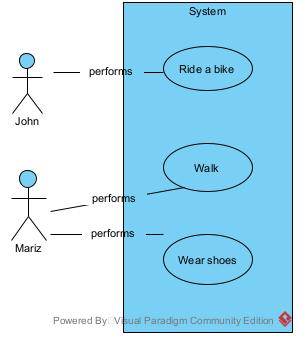
\includegraphics[scale=0.75]{Book-SSW565/jpg/ArchitectureModeling/Use Case Diagram1.jpg}
    \caption{\label{Figure::Use Case Diagram}Use Case Diagram}
\end{figure}


\section{Object Diagram}
The \textbf{Object Diagram} models a \textbf{specific scenario} of the user story. It represents actual instances of the classes at a given moment:
\begin{itemize}
    \item \textbf{John's Bike} is \textbf{directly associated} with him.
    \item \textbf{Maria owns shoes}, which she \textbf{needs for walking}.
    \item The \textbf{relationship between objects} is crucial: Maria \textbf{cannot walk without shoes}, reinforcing \textbf{dependency}.
    \item \textbf{Multiplicities} (one-to-one associations) are implied in the relationships to reflect real-world constraints.
\end{itemize}

The thought process behind this diagram was to provide \textbf{a snapshot} of how objects interact in the real world, helping to validate the correctness of the class relationships before formalizing them in the \textbf{Class Diagram}.

\begin{figure}[H]
    \centering
    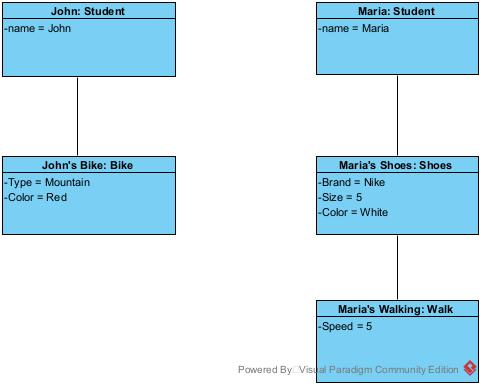
\includegraphics[scale=0.75]{Book-SSW565/jpg/ArchitectureModeling/Object Diagram1.jpg}
    \caption{\label{Figure::Object Diagram}Object Diagram}
\end{figure}

\section{Class Diagram}
The \textbf{Class Diagram} is the most detailed and structured representation of the system. It was designed using \textbf{three key relationships}:
\begin{itemize}
    \item \textbf{Generalization (Inheritance):} \texttt{Bike} and \texttt{Shoes} are both types of \texttt{TransportMode}, making use of \textbf{inheritance} to reduce redundancy.
    \item \textbf{Generalization (Inheritance):} \texttt{John} and \texttt{Maria} are both types of \texttt{Student}, making use of \textbf{inheritance} to reduce redundancy.
    \item \textbf{Aggregation:} A \texttt{Student} \textbf{uses} a \texttt{TransportMode} method but does not permanently own it (represented with a \textbf{hollow diamond}).
    \item \textbf{Composition:} \texttt{Student} \textbf{requires} \texttt{School} (depicted with a \textbf{filled diamond}), meaning a \texttt{Student} instance \textbf{cannot exist} without \texttt{School}.
\end{itemize}

This diagram refines the \textbf{structure of the system} by making clear distinctions between \textbf{inheritance, dependencies, and ownership relationships}, forming the blueprint for implementing the system in code.


\begin{figure}[h]
    \centering
    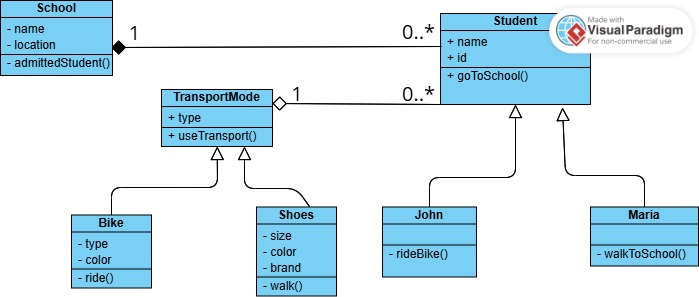
\includegraphics[scale=0.6]{Book-SSW565/jpg/ArchitectureModeling/Class_Diagram.jpg}
    \caption{\label{Figure::Class Diagram}Class Diagram}
\end{figure}

